\section{Experimental Analysis}

\subsection{Experimental Environment}
We use multiple tools and platforms for testing:
\begin{itemize}
    \item Tenderly platform: for contract deployment and trade simulation \url{https://dashboard.tenderly.co/explorer}
    \item Remix IDE: for contract compilation and initial testing \url{https://remix.ethereum.org}
    \item MetaMask: for testing network deployment
    \item Python matplotlib: for data visualization
\end{itemize}

Due to the limited testnet tokens, in this thesis we used tenderly for simulated transactions, which can get relevant detailed transaction information, and for each simulated transaction we performed 5 times to get the following average data to prevent chance situations.

\subsection{Gas Consumption Analysis}

\subsubsection{Error Handling Mechanisms}
Firstly, we tested the gas cost data for the three methods assert, require, revert for version 0.7.0 and 0.8.0 to get the following graphs:

\begin{figure}[h]
    \centering
    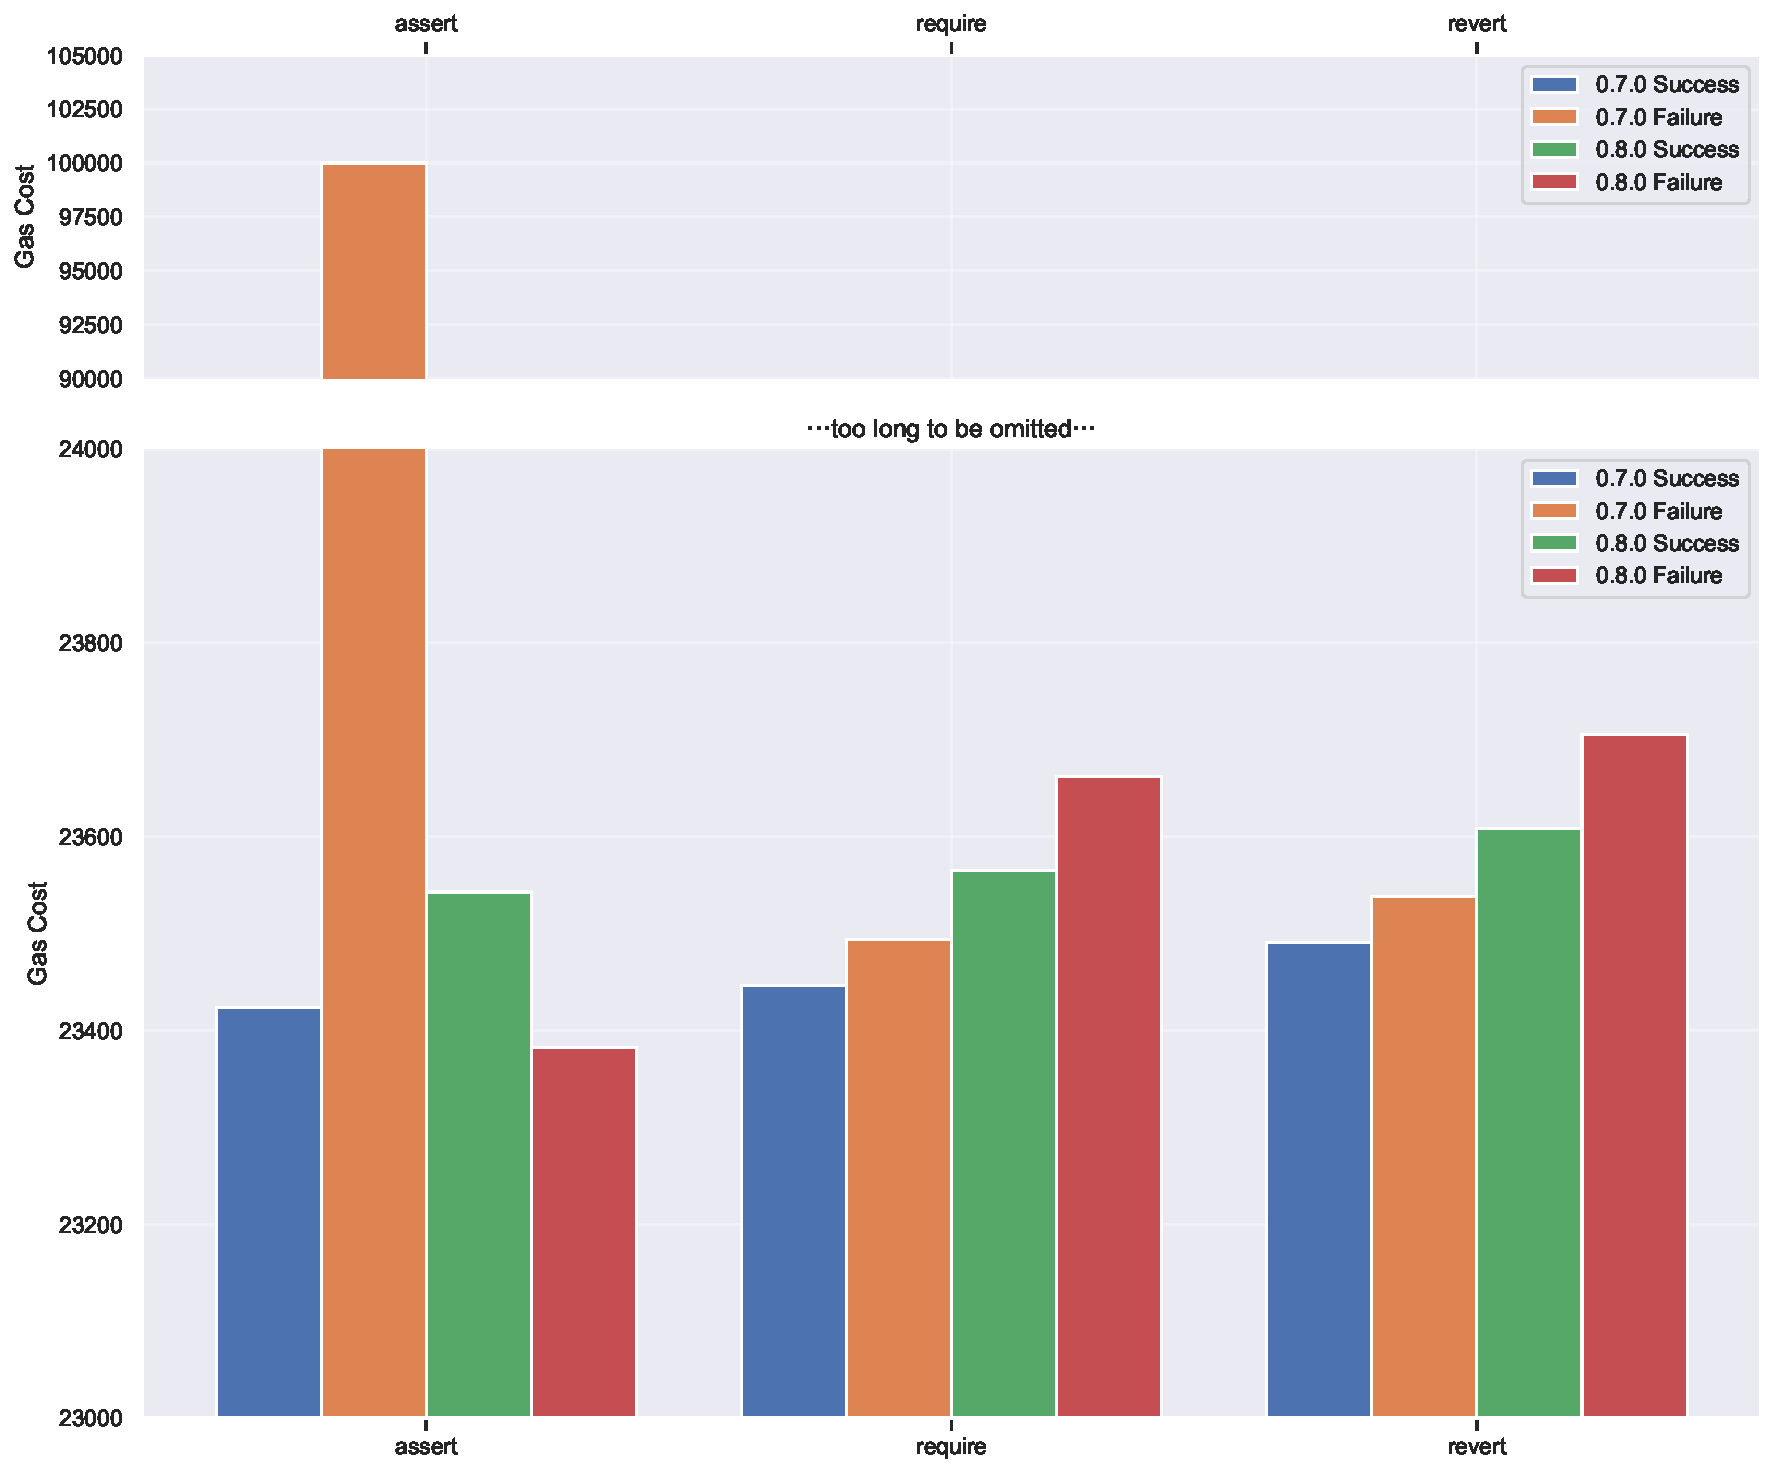
\includegraphics[width=0.8\textwidth]{figures/version_comparison.pdf}
    \caption{Gas Consumption Comparison Across Versions}
    \label{fig:version_comparison}
\end{figure}

We can see that failures tend to consume more gas than successes, this is due to the fact that the rollback operation after a failure consumes a certain amount of gas fee, due to the extra security checks added to these functions in version 0.8.0. The compiler generates more opcodes to handle boundary cases, so higher versions consume more gas for the same state, but we found that failing an assert transaction consumes all the gas in versions below 0.8.0, so developers should be more willing to spend a little bit more gas to get a more secure review mechanism to avoid excessive losses.

\subsubsection{Modifier vs Direct Validation}
Next, we also compared the difference in gas fee between using conditional validation directly in modifiers and functions, and got the following results:

\begin{figure}[h]
    \centering
    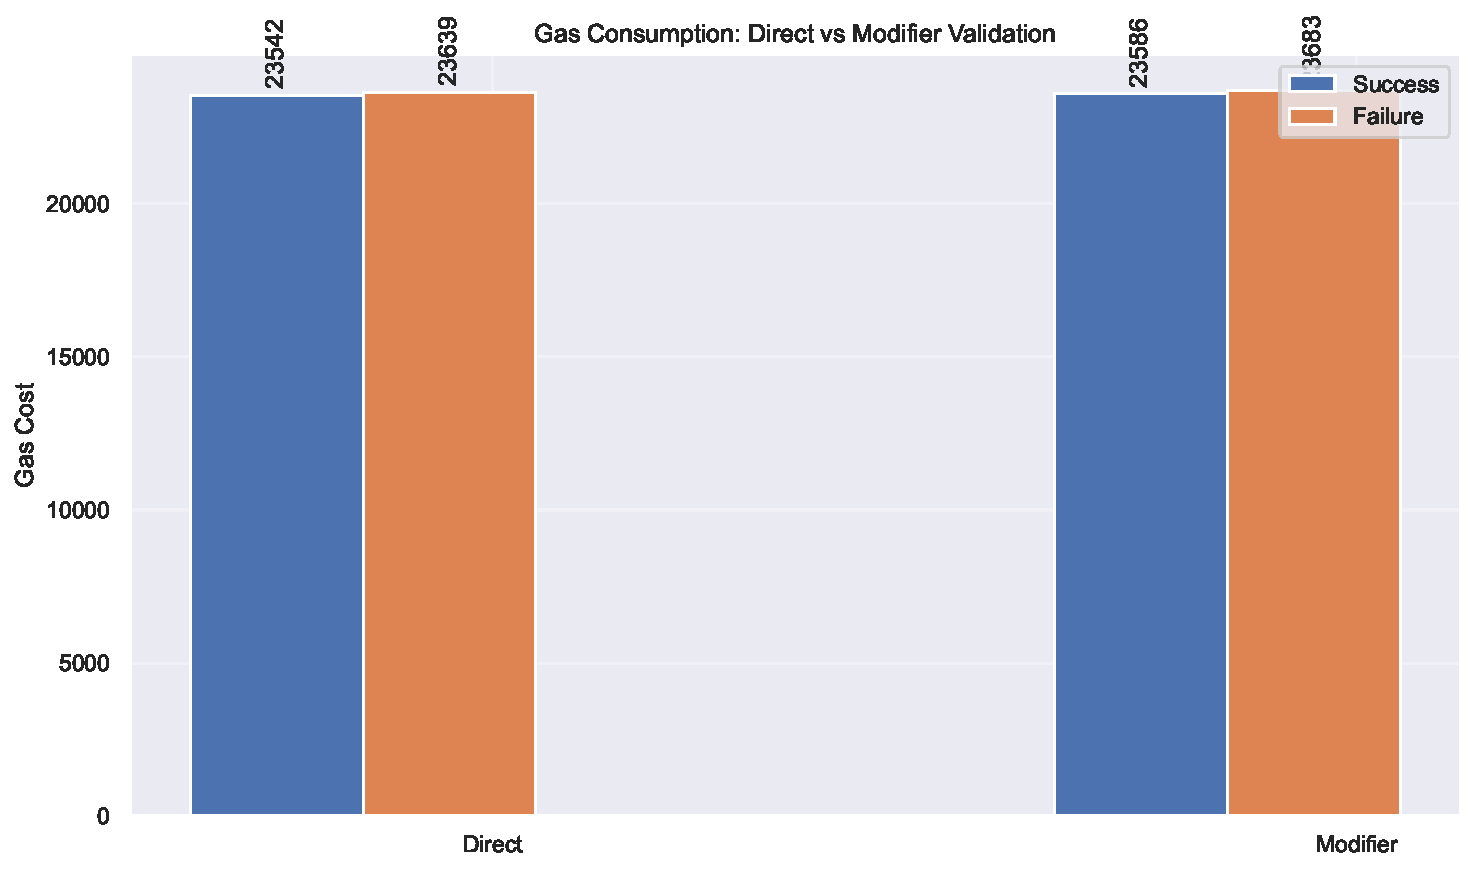
\includegraphics[width=0.8\textwidth]{figures/modifier_comparison.pdf}
    \caption{Gas Consumption: Modifier vs Direct Validation}
    \label{fig:modifier_comparison}
\end{figure}

We can see that although modifiers consume a little bit more, this is due to the fact that modifiers are essentially code inlining, and the compiler will insert the modifier code directly into the function. The final compiled bytecode is very similar, except for the extra jump instruction. Usually it only consumes about 20-50 gas more, but in view of the advantages of modifiers analysed above, this article suggests that they can all be expressed as modifiers, unless there are too many a priori conditions, and nesting modifiers in multiple layers may lead to errors, so we can use in-function conditions.

\subsubsection{Arithmetic Safety Mechanisms}
Since the problem of overflow above and below a function is very serious and can lead to contractually fatal errors, we have analysed the cost of gas consumed by safely adding and subtracting maths, and the results are as follows:

\begin{figure}[h]
    \centering
    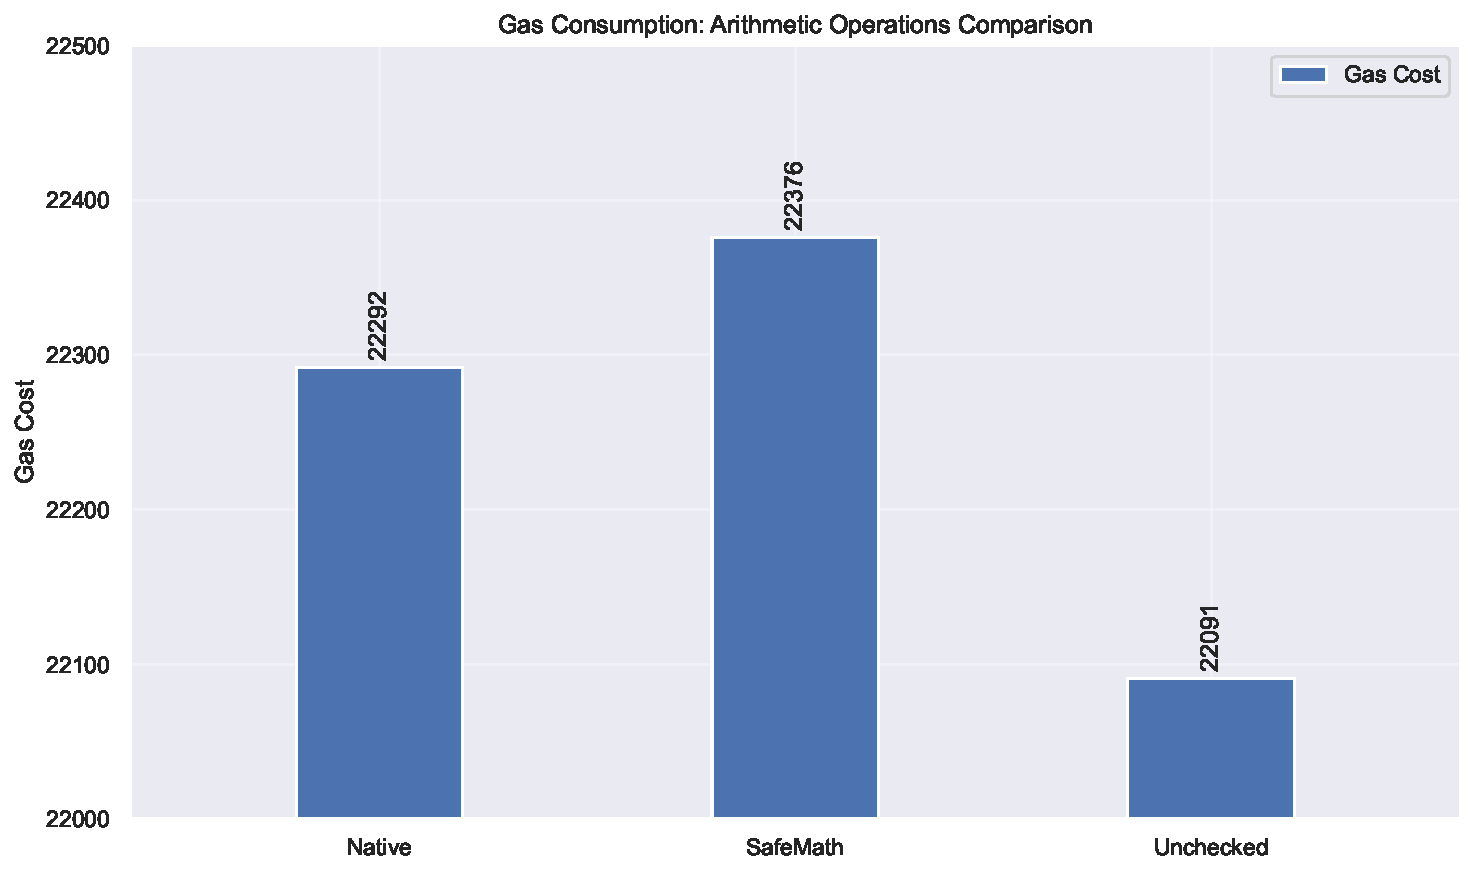
\includegraphics[width=0.8\textwidth]{figures/arithmetic_comparison.pdf}
    \caption{Gas Consumption: Arithmetic Operations Comparison}
    \label{fig:arithmetic_comparison}
\end{figure}

Since we are using version 0.8.0 or above, the compiler has been optimized, although it is not as big as the above comparative analysis of the gas difference, but the size of the gas cost can still reflect the performance of different methods, as we said above, unchecked consumes the smallest cost, safemath consumes the largest cost.

\subsubsection{ETH Transfer Methods}
In Ether smart contracts, ETH is closely related to the method of sending ETH, so we have also analyzed:

\begin{figure}[h]
    \centering
    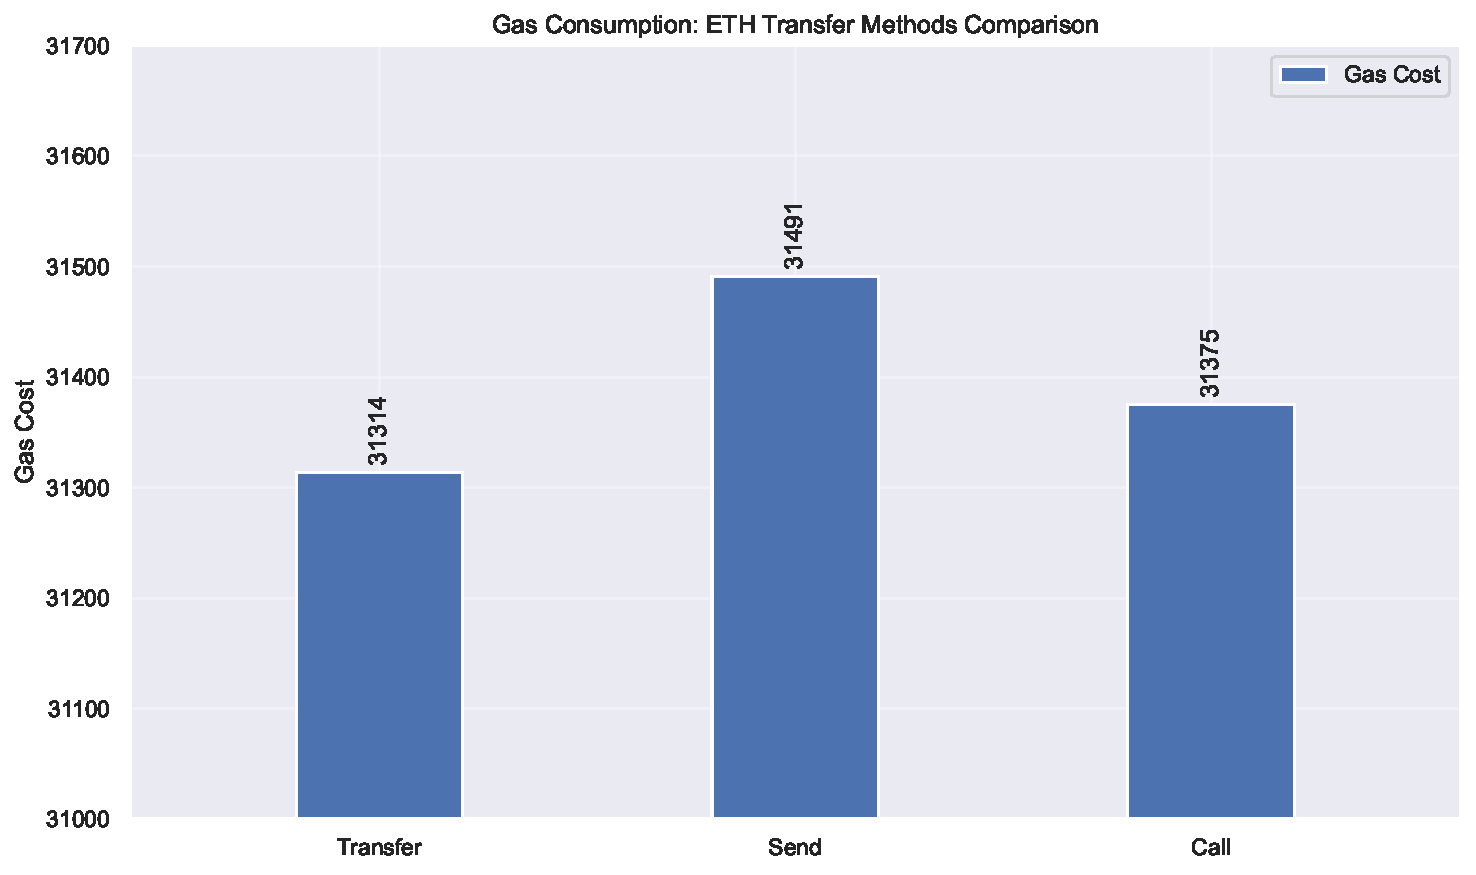
\includegraphics[width=0.8\textwidth]{figures/transfer_comparison.pdf}
    \caption{Gas Consumption: ETH Transfer Methods Comparison}
    \label{fig:transfer_comparison}
\end{figure}

The reason that transfer is lowest is that we use a fixed sequence of opcodes, which the compiler can optimize, and do not need to handle return values. Failure is rolled back directly without additional error handling logic, whereas send needs to handle boolean return values and includes an additional return value checking mechanism.